% TODO L08 REQUIREMENTS

\ifuniversity{tubs}{\date{December 3, 2024}}

\author{Thomas Thüm}
\lecture{Requirements}{requirements}

\begin{frame}{\insertsubtitle}
	\hprojectcartoon{01}{how the customer explained it}
	\hprojectcartoon{02}{how the project leader understood it}
	\alt<3->{%
		\projectcartoon{03}{how the analyst designed it}
		\projectcartoon{04}{how the programmer implemented it}
	}{%
		\hprojectcartoon{03}{how the analyst designed it}
		\hprojectcartoon{04}{how the programmer implemented it}
	}%
	\uncover<2->{\hprojectcartoon{13}{what the customer really needed}}
\end{frame}

\section{Introduction to Requirements}
\subsection{User Requirements}
\begin{frame}{\insertsubsection\ \deutsch{Benutzeranforderungen}}
	\begin{fancycolumns}
		\begin{definition}{User Requirement \mysource{\sommerville}}
			\mycite{User requirements are statements, in a natural language plus diagrams, of what services the system is expected to provide to system users and the constraints under which it must operate. The user requirements may vary from broad statements of the system features required to detailed, precise descriptions of the system functionality.}
		\end{definition}
		\begin{note}{User Requirements Document \deutsch{Lastenheft}}
			System description from user's point of view. What? For what? \deutsch{Was? Wofür?}
		\end{note}
		\nextcolumn
		\begin{example}{Example}
			The Corona app should track contacts by means of random IDs and should store them locally for two weeks.
		\end{example}
		\begin{example}{Example}
			If a user has a positive test result, he or she can inform tracked contacts about their increased risk by means of a QR code.
		\end{example}
	\end{fancycolumns}
\end{frame}

\begin{frame}[b]
	\begin{fancycolumns}
		\pic[width=\linewidth,trim=0 100 0 0,clip]{people/tony-hoare}
		\vspace{-7mm}
		
		\begin{note}{Tony Hoare (1969) \mysource{\href{https://dl.acm.org/doi/10.1145/363235.363259}{Hoare 1969}}}
			\mycite{The most important property of a program is whether it accomplishes the intention of its user.}
		\end{note}
	\end{fancycolumns}
\end{frame}

\subsection{System Requirements}
\begin{frame}{\insertsubsection\ \deutsch{Systemanforderungen}}
	\begin{fancycolumns}
		\begin{definition}{System Requirement \mysource{adapted from \sommerville}}
			System requirements are more detailed descriptions of the software system’s functions, services, and operational constraints. The system requirements document (aka.\ functional specification) should define exactly what is to be implemented. It may be part of the contract between the system buyer and the software developers.
		\end{definition}
		\begin{note}{System Requirements Document \deutsch{Pflichtenheft}}
			System description from technical point of view. How? Whereby? \deutsch{Wie? Womit?}
		\end{note}
		\nextcolumn
		\begin{example}{Example}
			If two devices are within a distance of 2m for at least 15 minutes they exchange their IDs via Bluetooth.
		\end{example}
		\begin{example}{Example}
			After IDs have been exchanged, they are stored for two weeks.
		\end{example}
		\begin{example}{Example}
			A new ID is generated every 24 hours and old IDs are stored for two weeks.
		\end{example}
	\end{fancycolumns}
\end{frame}

\subsection{Functional Requirements}
\begin{frame}{\insertsubsection}
	\begin{fancycolumns}
		\begin{definition}{Functional Requirement \mysource{\sommerville}}
			\mycite{Functional requirements are statements of services the system should provide, how the system should react to particular inputs, and how the system should behave in particular situations. In some cases, the functional requirements may also explicitly state what the system should not do.}
		\end{definition}
	\end{fancycolumns}
\end{frame}

\subsection{Non-Functional Requirements}
\begin{frame}{\insertsubsection}
	\begin{fancycolumns}
		\begin{definition}{Non-Functional Requirement \mysource{\sommerville}}
			\mycite{Non-functional requirements are constraints on the services or functions offered by the system. They include timing constraints, constraints on the development process, and constraints imposed by standards. Non-functional requirements often apply to the system as a whole rather than individual system features or services.}
		\end{definition}
		%\myexample{Generic Examples}{reliability, response time, memory consumption}
		\begin{note}{Note}
			often more critical than functional requirements
		\end{note}
		\nextcolumn
		\begin{example}{Example}
			The app consumes less than 10MB of RAM.
		\end{example}
		\begin{example}{Example}
			The app has no access to private data of the user.
		\end{example}
		\begin{example}{Example}
			The app conforms to the GDPR. \deutsch{DSGVO}
		\end{example}
		\begin{example}{Example}
			The source code of the app is open source.
		\end{example}
	\end{fancycolumns}
\end{frame}

\begin{frame}
	\centering
	\slideMindmapNonFunctionalRequirements
\end{frame}

\subsection{Structure of a Requirements Document}
\begin{frame}{\insertsubsection}
	\begin{definition}{Typical Structure \mysource{\sommerville}}
		\setlength\tabcolsep{1mm}
		\begin{tabularx}{\textwidth}{rX}
			\emph{Preface} & expected readers, version history\\
			\emph{Introduction} &  motivation/needs, collaboration with other system, strategic objectives\\
			\emph{Glossary} & technical terms\\
			\emph{User Requirements Definition} & functional and non-functional user requirements\\
			\emph{System Architecture} & distribution of functions across system modules, potential reuse\\
			\emph{System Requirements Specification} & detailed requirements, interfaces to other systems\\
			\emph{System Models} & graphical models illustrating the system with its environment\\
			\emph{System Evolution} & anticipated changes due to hardware evolution or changing needs\\
			\emph{Appendices} & hardware and database requirements, minimal/optimal system configuration\\
			\emph{Index} & index of diagrams/functions/terms/\ldots
		\end{tabularx}
	\end{definition}
\end{frame}

\lessonslearned{
	\item What kind of requirements exist and why?
	\item User and System Requirements Document \deutsch{Lasten- und Pflichtenheft}
	\item Next: Where do requirements come from?
}{
	\item \sommerville\mychapter{2.2.1}\mypages{54--55}
	\item \sommerville\mychapter{4.1}\mypages{101--111}
	\item \sommerville\mychapter{4.4.4}\mypages{126--128}
}{
	\begin{enumerate}
		\item Form groups of 2--3 students
		\item On your own: write down 1--2 own examples for a requirement
		\item Group work: classify each others requirements in groups of 2--3 students
		\item Try to find an example for each of the four categories: functional, non-functional (product, organizational, and external)
	\end{enumerate}
	Hint: Keep written requirements for a later interaction
}

\section{Elicitation of Requirements}
\subsection{Imprecise Requirements}
\begin{frame}{\insertsubsection}
	\begin{fancycolumns}[animation=none]
		\begin{note}{\sommerville:}
			\mycite{Imprecision in the requirements specification can lead to disputes between customers and software developers. It is natural for a system developer to interpret an ambiguous requirement in a way that simplifies its implementation. Often, however, this is not what the customer wants. New requirements have to be established and changes made to the system. Of course, this delays system delivery and increases costs.}
		\end{note}
		\nextcolumn
		\renewcommand{\projectcartoonwidth}{.3}
		\pause\hprojectcartoon{02}{how the project leader understood it}
		\hprojectcartoon{04}{how the programmer implemented it}
		\hprojectcartoon{13}{what the customer really needed}
	\end{fancycolumns}
\end{frame}

\subsection{Complete and Consistent Requirements}
\begin{frame}{\insertsubsection}
	\begin{fancycolumns}
		\begin{definition}{Completeness and Consistency \mysource{\sommerville}}
			\mycite{Ideally, the functional requirements specification of a system should be both complete and consistent. \emph{Completeness} means that all services and information required by the user should be defined. \emph{Consistency} means that requirements should not be contradictory.}
		\end{definition}	
		\begin{note}{Further Desired Properties}
			clear, easy to understand, unambiguous, correct, verifiable, prioritized, changeable, traceable %\deutsch{eindeutig, korrekt, überprüfbar, priorisiert, änderbar, nachvollziehbar}
		\end{note}
		\nextcolumn
		\begin{example}{Often not Feasible in Practice}
			mistakes, omission, implicit knowledge, many stakeholders \deutsch{Akteure} with different backgrounds / expectations / inconsistent needs
		\end{example}
	\end{fancycolumns}
\end{frame}

\begin{frame}[b]
	\begin{fancycolumns}
		\vspace{2mm}
		\pic[width=\linewidth,trim=0 175 0 75,clip]{people/fred-brooks}
		\vspace{-7mm}
		
		\begin{note}{Fred Brooks (1931--2022) \mysource{\href{https://ieeexplore.ieee.org/document/1663532}{Brooks 1987}}}
			\mycite{Much of the essence of building a program is in fact the debugging of the specification.}
		\end{note}
	\end{fancycolumns}
\end{frame}

\subsection{Requirements Engineering Process}
\begin{frame}{\insertsubsection} % TODO define term requirements engineering?
	\begin{fancycolumns}[columns=3,widths={80}]
		\begin{definition}{Requirements Elicitation and Analysis \mysource{adapted from \sommerville}}
			Requirements elicitation and analysis is the process of deriving the system requirements through observation of existing systems, discussions with potential users, or development of prototypes. \deutsch{Anforderungsermittlung und -analyse} 
		\end{definition}
		\nextcolumn
		\nextcolumn
	\end{fancycolumns}
	\begin{fancycolumns}[columns=3,widths={10,80,10}]
		\nextcolumn
		\begin{definition}{Requirements Specification \mysource{\sommerville}}
			\mycite{Requirements specification is the process of writing down the user and system requirements in a requirements document (aka. requirements specification).} \deutsch{Anforderungsspezifikation}
		\end{definition}
		%Requirements specification is the activity of translating the information gathered during requirements analysis into a document that defines a set of requirements (incl. user and system requirements).
		\nextcolumn
	\end{fancycolumns}
	\begin{fancycolumns}[columns=3,widths={10,10,80}]
		\nextcolumn
		\nextcolumn
		\begin{definition}{Requirements Validation \mysource{\sommerville}}
			\mycite{Requirements validation  is an activity that checks the requirements for realism, consistency, and completeness.} \deutsch{Anforderungsvalidierung}
		\end{definition}
	\end{fancycolumns}
\end{frame}
% TODO replace picture with tikz? simplify it? add in SE2 in more detail?
%\pause\pic[width=\linewidth]{sommerville/p55-f2.4}

\subsection{Why is Requirements Elicitation so Hard?}
\begin{frame}{\insertsubsection}
	\begin{fancycolumns}[animation=none,widths={66}]
		\begin{example}{}
			\begin{itemize}
				\item Stakeholders have difficulties to articulate what they want
				\item Stakeholders do not know what is (in)feasible
				\item Implicit knowledge and jargon in the customer's domain
				\item Dynamic business environment (e.g., new stakeholders)
			\end{itemize}
		\end{example}
	\end{fancycolumns}
\end{frame}

\subsection{Example Dialog by Ludewig and Lichter}
\begin{frame}{\insertsubsection}
	\begin{fancycolumns}[animation=none]
		\begin{itemize}
			\item At the morning you unlock the door at the main entrance?
			\item Every morning?
			\item Even at the weekend?
			\item And during the plant shutdown?
			\item And if you are sick or in holidays?
			\item And if Mr. X is off?
			\item What does \mycite{morning} mean?
		\end{itemize}
		\nextcolumn\vspace{5mm}
		\begin{itemize}
			\item Yes, as I said.
			\item Of course.
			\item No, at weekend the entrance remains closed.
			\item Clearly, it is then closed as well.
			\item Mr. X opens the door in this case.
			\item Then, a client knocks at the window to tell that the door is closed.
			\item \ldots
		\end{itemize}
	\end{fancycolumns}
	\vspace{5mm}
	
	Source: \ludewiglichter
	
	\href{https://youtu.be/NEUNEmJQGMw?t=1156}{Skit on Youtube (in German)}
\end{frame}

\subsection{Requirements Elicitation Techniques}
\begin{frame}{\insertsubsection}
	\begin{fancycolumns}[keep]
		\begin{definition}{Techniques for Requirement Elicitation}
			\begin{itemize}
				\item Open interviews: talk to users what they do
				\item Closed interviews: stakeholders answer predefined questions
				\item Ethnography: observation of stakeholder's work
				\item Prototyping
				\item Feedback loops
			\end{itemize}
		\end{definition}
		\nextcolumn
		\begin{note}{\sommerville:}
			\mycite{You need to spend time understanding how people work,
				what they produce, how they use other systems, and how they may need to change to accommodate a new system.}
		\end{note}
		\begin{example}{In Practice}
			Combinations of numerous techniques used
		\end{example}
	\end{fancycolumns}
\end{frame}

\subsection{Requirements Validation}
\begin{frame}{\insertsubsection}
	\begin{fancycolumns}[animation=none,widths={75}]
		\begin{note}{Motivation}
			The later problems with requirements are detected, the more costly it will be to fix them.
		\end{note}
		\begin{definition}{Requirements Validation}
			\setlength\tabcolsep{1mm}
			\begin{tabularx}{\textwidth}{rX}
				\emph{Validity checks} & do requirements (still) reflect real needs?\\
				\emph{Consistency checks} & are there contradictory/redundant requirements?\\
				\emph{Completeness checks} & are all functions and constrains documented?\\
				\emph{Realism checks} & is it feasible within budget and schedule?\\
				\emph{Verifiability} & can we test the requirements?
			\end{tabularx}
			
			~\\Checked by reviews, prototyping, and test-case creation
		\end{definition}
	\end{fancycolumns}
\end{frame}


\lessonslearned{
	\item Desired properties for requirements
	\item Requirements engineering process?
	\item Techniques for requirements elicitation
	\item Next: How to document requirements graphically?
}{
	\item \sommerville\mychapter{4.2--4.3}\mypages{111--119}
	\item \sommerville\mychapter{4.5}\mypages{129f}
}{
	\begin{enumerate}% TODO animation of practical tasks does not work. remove animations everywhere?
		\item Form groups of 2--3 students
		\item On your own: reconsider your written examples and write down improved versions
		\item Group work: let your colleagues guess what property you aimed to improve
	\end{enumerate}
	Hint: Recap on desired properties: complete, consistent, clear, easy to understand, unambiguous, correct, verifiable, prioritized, changeable, traceable
}

\section{Documentation of Requirements}
\subsection{Natural Language Specification}
\begin{frame}{\insertsubsection}
	\begin{fancycolumns}[widths={55}]
		\begin{definition}{}
			\begin{itemize}
				\item used since 1950s
				\item since programmer is not necessarily the user
			\end{itemize}
		\end{definition}
		\begin{example}{Style Guidelines}
			\begin{itemize}
				\item one or two short sentences of natural language
				\item one message per sentence
				\item use active voice (e.g., \mycite{the system \ldots})
				\item consistent use of language (i.e., avoid synonyms)
				\item use shall for mandatory and should for desirable requirements
				\item use text highlighting
				\item avoid jargon, abbreviations, acronyms
				\item provide a rationale
			\end{itemize}
		\end{example}
		\nextcolumn
		\begin{note}{Pros}
			\begin{itemize}
				\item expressive
				\item intuitive
				\item universal
			\end{itemize}
		\end{note}
		\begin{note}{Cons}
			\begin{itemize}
				\item vague \deutsch{vage}
				\item ambiguous \deutsch{mehrdeutig}
				\item interpretation depends on reader's background
			\end{itemize}
		\end{note}
	\end{fancycolumns}
\end{frame}

\subsection{Structured Specifications}
\begin{frame}{\insertsubsection}
	\begin{fancycolumns}[widths={55}]
		\begin{definition}{}
			\begin{itemize}
				\item use of templates rather than free-form text
				\item distinguishes between function, description, input (origin), output (destination), pre- and postconditions, side effects, rationale, dependencies to other requirements, \ldots
				\item or any subset thereof
				\item user stories are typically structured specifications
			\end{itemize}
		\end{definition}
		\begin{example}{Example}
			\setlength\tabcolsep{1mm}
			\begin{tabularx}{\textwidth}{rX}
				Function & Exchange of IDs\\
				Description & Two devices send their IDs to each other.\\
				Precondition & Devices have been within a distance of 2m for at least 15 minutes.\\
				Postcondition & IDs are stored in the local database.\\
				Rationale & Contact tracing requires to temporarily identify the device of contacts.
			\end{tabularx}
		\end{example}
		\nextcolumn
		\begin{note}{Pros}
			\begin{itemize}
				\item {\color{gray} expressive}
				\item {\color{gray} intuitive}
				\item information easier to find
				\item less likely to forget certain information (e.g., rationale)
			\end{itemize}
		\end{note}
		\begin{note}{Cons}
			\begin{itemize}
				\item {\color{gray} vague}
				\item {\color{gray} ambiguous}
				\item {\color{gray} interpretation depends on reader's background}
				\item same structure can be too restrictive
				\item multiple structures can be confusing
			\end{itemize}
		\end{note}
	\end{fancycolumns}
\end{frame}

\subsection{Use Case Diagrams}
\begin{frame}[label=usecaseslide]{\insertsubsection\ \normalsize(since 1993)}
	\begin{fancycolumns}[animation=none]
		\begin{definition}{Use Case Diagram \deutsch{Anwendungsfalldiagramm}}
			Use case diagrams are a means to capture the requirements of systems, i.e., what systems are supposed to do. The key concepts specified in this diagram are actors, use cases, and subjects:%\\~
			\begin{itemize}
				\item Each \emph{subject} represents a system under consideration to which the use case applies. \deutsch{System}
				\item Each users and any other system that may interact with a subject is represented as an \emph{actor}. \deutsch{Akteur}
				\item A \emph{use case} is a specification of behavior in terms of verb and noun. \deutsch{Anwendungsfall}
			\end{itemize}
			\mysource{adapted from \umlspec}
		\end{definition}
		\nextcolumn
		%\posthandout{\pic[width=\linewidth,trim=0 50 25 40,clip]{blackboard/blackboard_use_case1_23_24}}
		%\posthandout{\pic[page=44,width=\linewidth,trim={.5\width} {.1\height} {.02\width} {.2\height},clip]{se09-requirements-print}}
	\end{fancycolumns}
\end{frame}

\begin{frame}{Example}
\end{frame}

\subsection{Include and Extend Relationships}
\begin{frame}[label=includeandextendslide]{\insertsubsection}
	\begin{fancycolumns}[animation=none]
		\begin{definition}{Include Relationship}
			\textbf{Motivation}: make common parts of multiple use cases explicit%\\[1mm]
			
			\textbf{Relationship}: a \emph{base use case} may define an include relationship to an \emph{included use case}%\\[1mm]
			
			\textbf{Meaning}: included use case is always executed when the base use case is
		\end{definition}
		\begin{definition}{Extend Relationship}
			\textbf{Motivation}: make explicit that some use cases only happen under certain circumstances%\\[1mm]
			
			\textbf{Relationship}: an \emph{extend use case} may define an extend relationship to a \emph{base use case}%\\[1mm]
			
			\textbf{Meaning}: when the base use case is executed, the extend use case may or may not be executed
		\end{definition}
		\nextcolumn
		%\posthandout{\pic[page=53,width=\linewidth,trim=225 20 15 50,clip]{se02-requirements-print}}
		%\posthandout{\pic[page=46,width=\linewidth,trim={.5\width} {.2\height} {.02\width} {.2\height},clip]{se09-requirements-print}}
	\end{fancycolumns}
\end{frame}

% TODO add rules for use case diagrams

% TODO discuss advantages/disadvantages of use case diagrams

% TODO combination of textual and visual requirements

\pictureframe{
	\pic[width=\paperwidth]{emotions/walking-on-water}
}{
	\vspace{65mm}
	\begin{note}{Edward V. Berard (1993) \mysource{\href{https://en.wikiquote.org/wiki/Edward_V._Berard}{wikiquote.org}}}
		\mycite{Walking on water and developing software from a specification are easy if both are frozen.}
	\end{note}
}

\lessonslearned{
	\item Natural language and structured specification of requirements
	\item Graphical specification with use case diagrams \deutsch{Anwendungsfalldiagramme}
	\item Next: How to model the system behavior in more detail?
}{
	\item \sommerville\mychapter{4.4}\mypages{120--126}
	\item \sommerville\mychapter{5.2.1}\mypages{144--146}
	\item \umlspec\mychapter{18}
}{
	Quiz in Stud.IP
	\lectureqr{08}
}

%\faq{
	%	\item
	%}{
	%	\item
	%}{
	%	\item
	%}

\mode<beamer>{
	\addtocounter{framenumber}{-1}
	\begin{frame}{\inserttitle}
		\lectureseriesoverview[\insertlecturenumber]
	\end{frame}

	%\addtocounter{framenumber}{-1}
	%\againtitle % TODO does not work as we have redefined maketitle
}


% TODO L09 SYSTEM MODELING

\ifuniversity{tubs}{\date{December 10, 2024}}

\author{Thomas Thüm}
\lecture{System Modeling}{modeling}

% TODO blackboard on graphical notation: use case vs system vs activity vs state

\begin{frame}{\insertsubtitle}
	\hprojectcartoon{01}{how the customer explained it}
	\hprojectcartoon{02}{how the project leader understood it}
	\alt<3->{%
		\projectcartoon{03}{how the analyst designed it}
		\projectcartoon{04}{how the programmer implemented it}
	}{%
		\hprojectcartoon{03}{how the analyst designed it}
		\hprojectcartoon{04}{how the programmer implemented it}
	}%
	\uncover<2->{\hprojectcartoon{13}{what the customer really needed}}
\end{frame}

\section{Introduction to Modeling}
\subsection{Motivation for Modeling}
\begin{frame}{\insertsubsection}
	\begin{fancycolumns}
		\begin{note}{\umluserguide:}
			\mycite{A successful software organization is one that consistently deploys \emph{quality software} that meets the needs of its users. An organization that can develop such software in a \emph{timely and predictable} fashion, with an \emph{efficient and effective use of resources}, both human and material, is one that has a sustainable business.
				
				[...]
				
				Modeling is a central part of all the activities that lead up to the deployment of good software. We build models to \emph{communicate} the desired structure and behavior of our system. We build models to \emph{visualize and control} the system's architecture. We build models to better \emph{understand} the system we are building, often exposing opportunities for \emph{simplification and reuse}. And we build models to \emph{manage risk}.}
		\end{note}
		\nextcolumn
		\begin{note}{\umluserguide:}
			\mycite{We build models of complex systems because we cannot comprehend such a system in its entirety.}
		\end{note}
	\end{fancycolumns}
\end{frame}

\begin{frame}[b]{Recap: Software Engineering vs Programming}
	\slideSEvsProgramming
\end{frame}

\begin{frame}
	\begin{fancycolumns}
		\pic[width=\linewidth,trim=0 300 0 80,clip]{people/bjarne-stroustrup}
		\vspace{-7mm}
		
		\begin{note}{Bjarne Stroustrup (2000) \mysource{\cpp}}
			\mycite{The most important single aspect of software development is to be clear about what you are trying to build.}
		\end{note}
	\end{fancycolumns}
\end{frame}

\subsection{What is System Modeling?}
\begin{frame}{\insertsubsection}
	\begin{fancycolumns}
		\begin{definition}{System Modeling \mysource{\sommerville}}
			\mycite{\emph{System modeling} is the process of developing abstract models of a system, with each model presenting a different view or perspective of that system. [...] Models are used during the requirements engineering process to help derive the \emph{detailed requirements} for a system, during the design process to \emph{describe the system to engineers} implementing the system, and after implementation to \emph{document the system}’s structure and operation.}
		\end{definition}
	\end{fancycolumns}
\end{frame}

\subsection{What is a Model?}
\begin{frame}{\insertsubsection}
	\begin{fancycolumns}
		\begin{definition}{\umluserguide:}
			\mycite{A \emph{model} is a simplification of reality.}
		\end{definition}
		\begin{definition}{\sommerville:}
			\mycite{A \emph{model} is an abstract view of a system that deliberately ignores some system details.}
		\end{definition}
		\begin{note}{{Goals of Models \mysource{\umluserguide}}}
			\begin{itemize}
				\item visualize a system as it is (wanted)
				\item specify the structure or behavior of a system
				\item template to guide construction of a system
				\item document the decisions we have made
			\end{itemize}
		\end{note}
		\nextcolumn
		\begin{note}{\sommerville:}
			\mycite{It is important to understand that a system model is \emph{not a complete representation} of system. It purposely leaves out detail to make it \emph{easier to understand}. A model is an abstraction of the system being studied rather than an alternative representation of that system. A representation of a system should maintain all the information about the entity being represented. An abstraction \emph{deliberately simplifies a system} design and picks out the most salient characteristics.}
		\end{note}
	\end{fancycolumns}
\end{frame}

\subsection{What Language to Use for Modeling?}
\begin{frame}{\insertsubsection}
	\begin{fancycolumns}
		\myexample{Towards a Common Language}{
			\begin{itemize}
				\item Natural language? hard to abstract from details, already used in requirements
				\item Programming language? unfamiliar to people without programming skills in that language, too early to decide for the programming language
				\item Textual language? harder to understand
				\item Graphical language? makes use of our visual abilities, requires common understanding
				\item Problem: engineers need to be aware of all languages being used
				\item Solution: use a graphical language independent of company and domain
			\end{itemize}
		}
	\end{fancycolumns}
\end{frame}

% TODO new slides on History of Modeling Languages?

\xkcdframe{927} % 14+1 standards

\subsection{The Unified Modeling Language (UML)}
\begin{frame}{\insertsubsection}
	\begin{fancycolumns}
		\begin{definition}{UML \mysource{\umlrefman}}
			\mycite{The Unified Modeling Language (UML) is a general-purpose visual modeling language that is used to specify, visualize, construct, and document the artifacts of a software system.}
		\end{definition}
		\pause
		\begin{note}{\umluserguide:}
			\mycite{Modeling yields an understanding of a system. No one model is ever sufficient. Rather, you often need multiple models that are connected to one another [...].}
		\end{note}
	\end{fancycolumns}
\end{frame}

\subsection{Different Kinds of UML Diagrams}
\begin{frame}{\insertsubsection}
	\begin{fancycolumns}
		\begin{definition}{Structure Diagrams \deutsch{Strukturdiagramme}}
			\mycite{\emph{Structure diagrams} show the static structure of the objects in a system. That is, they depict those elements in a specification that are irrespective of time. The elements in a structure diagram represent the meaningful concepts of an application, and may include abstract, real-world and implementation concepts.}\mysource{\umlspec}
		\end{definition}	
		\nextcolumn
		\begin{definition}{Behavior Diagrams \deutsch{Verhaltensdiagramme}}
			\mycite{\emph{Behavior diagrams} show the dynamic behavior of the objects in a system, including their methods, collaborations, activities, and state histories. The dynamic behavior of a system can be described as a series of changes to the system over time.}\mysource{\umlspec}
		\end{definition}
	\end{fancycolumns}
\end{frame}
% TODO add paragraph on interaction diagrams?

\subsection{14 Types of UML Diagrams}
\begin{frame}{\insertsubsection\ \mytitlesource{\umlspec}}
	\only<-4>{\tikzset{notTaughtUMLDiagrams/.style={}}}%
	\only<-5|handout:0>{\slideMindmapUMLdiagrams{}{}{}{}{}{}{visible on={<2->}}{visible on=<3->}{visible on=<4->}}%
	\only<6|handout:0>{\slideMindmapUMLdiagrams{blue}{}{}{}{}{}{}{}{}}%
	\only<7->{\slideMindmapUMLdiagrams{blue}{red}{red}{}{}{}{}{}{}}%
	
	\uncover<5->{Six most important UML diagrams* discussed in this course
		
		*\tiny\href{https://dl.acm.org/doi/10.1145/1278201.1278205}{John Erickson and Keng Siau. 2007. Theoretical and practical complexity of modeling methods. Commun. ACM 50, 8 (August 2007), 46–51.}}
\end{frame}

% TODO talk about SysML? or at least mention in the slides?

\lessonslearned{
	\item System modeling
	\item Models as abstractions
	\item UML and its visual languages
	\item Next: How to model activities of a system?
}{
	\item[] \umluserguide\mychapter{1} --- great introduction to modeling
}{
	\begin{enumerate}
		\item Form groups of 2--3 students
		\item In isolation: Practice abstraction by sketching this lecture hall in \href{https://webuhr.de/timer-auf-1-minute/}{1 minute} (not more!).
		\item Groupwork: Show the sketch to your group and discuss what details are not shown in your visualizations. (5 min)
	\end{enumerate}
}

\section{Modeling Behavior with Activity Diagrams}
\xkcdframe{844}

\subsection{Activity Diagrams}
\begin{frame}{\insertsubsection}
	\begin{fancycolumns}[animation=none]
		\onlyhandout{\pic[page=3,width=\linewidth,trim=60 140 450 150,clip]{modeling/09-modeling_drawings}}
		\nextcolumn
		\begin{definition}{Activity Diagram \deutsch{Aktivitätsdiagramm}}
			An \emph{activity diagram} is a diagram visualizing activities and their order of execution. An activity diagram contains \emph{activities} (rounded box) that are connected by means of \emph{flows} (solid arrows). The execution begins at the \emph{initialization} (filled circle) and ends with the \emph{completion} node (bull's eye). \deutsch{Aktivität, Fluss, Startzustand, Endzustand}
		\end{definition}
		\pause%
		\begin{note}{Rules for Activity Diagrams}
			\begin{itemize}
				\item exactly one initialization node
				\item at least one activity
				\item every activity has one incoming and one outgoing flow
				\item every activity is reachable from initialization
				\item completion is reachable from every activity
			\end{itemize}
		\end{note}
		% What is the difference between activity and action? \umluserguide
	\end{fancycolumns}
\end{frame}

% TODO make sure that example contains activities (i.e., not only nouns)
\begin{frame}{Example of Sequential Activities}
	\onlyhandout{\pic[page=4,width=\linewidth,trim=60 80 80 120,clip]{modeling/09-modeling_drawings}}
\end{frame}

\subsection{Branching and Merging in Activity Diagrams}
\begin{frame}{\insertsubsection}
	\begin{fancycolumns}[animation=none]
		\onlyhandout{\pic[page=5,width=\linewidth,trim=60 120 450 150,clip]{modeling/09-modeling_drawings}}
		\nextcolumn
		\begin{definition}{{Branching and Merging \mysource{\umluserguide}}}
			\textbf{Motivation}: model control flow that depends on certain conditions (i.e., actions that may happen)
			
			\textbf{Branching}: A \emph{branch} has exactly one incoming and two or more outgoing flows. Each outgoing flow has a Boolean expression called \emph{guard}, which is evaluated on entering the branch. \deutsch{Verzweigung}
			
			\textbf{Merging}: A \emph{merge} has two or more incoming and exactly one outgoing flow. \deutsch{Zusammenführung}
		\end{definition}
		\pause
		\begin{note}{Further Rules for Activity Diagrams}
			\begin{itemize}
				\item guards on outgoing flows should not overlap (flow of control is unambiguous)
				\item guards should cover all possibilities (flow of control does not freeze)
				\item keyword \emph{else} possible for one guard \deutsch{sonst}
			\end{itemize}
		\end{note}
	\end{fancycolumns}
\end{frame}

\begin{frame}{Example of Conditional Activities}
	\onlyhandout{
		\pic[page=1,width=\linewidth,trim=60 80 80 150,clip]{modeling/09-modeling_drawings}
	}
\end{frame}

\subsection{Forking and Joining in Activity Diagrams}
\begin{frame}{\insertsubsection}
	\begin{fancycolumns}[animation=none]
		\onlyhandout{\pic[page=2,width=\linewidth,trim=60 140 450 120,clip]{modeling/09-modeling_drawings}}
		\nextcolumn
		\begin{definition}{{Forking and Joining \mysource{\umluserguide}}}
			\textbf{Motivation}: model concurrent control flows (i.e., activities that run in parallel)
			
			\textbf{Forking}: A \emph{fork} (thick horizontal or vertical line) has exactly one incoming and two or more outgoing flows. \deutsch{Gabelung}
			
			\textbf{Joining}: A \emph{join} (thick horizontal or vertical line) has two or more incoming and exactly one outgoing flow. \deutsch{Vereinigung}
		\end{definition}
		\pause
		\begin{note}{Further Rules for Activity Diagrams}
			\begin{itemize}
				\item branched paths must be merged eventually \deutsch{letztendlich}
				\item forked paths must be joined eventually
				\item only outgoing edges of branch nodes have guards
			\end{itemize}
		\end{note}
	\end{fancycolumns}
\end{frame}

	\begin{frame}{Example of Concurrent Activities}
		\onlyhandout{\pic[page=6,width=\linewidth,trim=60 100 10 120,clip]{modeling/09-modeling_drawings}}
	\end{frame}

\subsection{Swimlanes in Activity Diagrams}
\begin{frame}{\insertsubsection}
	\begin{fancycolumns}[animation=none]
		\onlyhandout{\pic[page=1,width=\linewidth,trim=60 100 150 150,clip]{modeling/09-modeling_drawings}}
		\nextcolumn
		\begin{definition}{{Swimlanes \mysource{\umluserguide}}}
			\textbf{Motivation}: group activities according to responsibilities
			
			\textbf{Swimlane}: An activity diagram may have no or at least two swimlanes. A \emph{swimlane} (rectangle) represents a high-level responsibility activities within an activity diagram. \deutsch{Verantwortlichkeitsbereiche}
		\end{definition}
		\pause
		\begin{note}{Further Rules for Activity Diagrams}
			\begin{itemize}
				\item each swimlane has a name unique within its diagram
				\item every activity belongs to exactly one swimlane
				\item only flows may cross swimlanes
			\end{itemize}
		\end{note}
	\end{fancycolumns}
\end{frame}

\begin{frame}{Recap: 14 Types of UML Diagrams\ \mytitlesource{\umlspec}}
	\slideMindmapUMLdiagrams{blue}{blue}{red}{}{}{}{}{}{}
\end{frame}


\lessonslearned{
	\item UML activity diagrams
	\item Branching and merging
	\item Forking and joining
	\item Swimlanes
	\item Next: How to model states of a system?
}{
	\item[] \umluserguide\mychapter{20}
	% less suited introduction: \sommerville, Chapter 5.1 (p.\ 141--144)
}{
	\begin{enumerate}
		\item Form groups of 2--3 students
		\item Draw a activity diagram for an instant messenger by yourself.
		\item It should contain at least one branch or fork. You are free to use swimlanes.
		\item Exchange your diagrams within your group and look for mistakes.
	\end{enumerate}
}

\section{Modeling Behavior with State Machines}
\subsection{Activity and State Machine Diagrams}
\begin{frame}{\insertsubsection}
	\begin{fancycolumns}
		\begin{note}{\umluserguide:}
			We can visualize the dynamics of execution in two ways: by emphasizing the flow of control from activity to activity (\emph{activity diagrams}) or by emphasizing the potential states and transitions among those states (\emph{state machine diagrams}).
		\end{note}
	\end{fancycolumns}
\end{frame}

\subsection{State Machine Diagrams}
\begin{frame}[label=statemachineslide]{\insertsubsection}
	\begin{fancycolumns}
		\begin{definition}{State Machine Diagram \deutsch{Zustandsdiagramm}}
			A \emph{state machine diagram} specifies the sequences of states the (a part of) the system goes through during its lifetime in response to events, together with its responses to those events. Every \emph{state} (rectangle with rounded corners) is characterized by a condition or situation. An \emph{event} is an occurrence of a stimulus that can trigger a state transition. A \emph{transition} (solid arrow) is a relationship between two states. \deutsch{Zustand, Ereignis, Zustandsübergang} \mysource{adapted from \umluserguide}
		\end{definition}
		\pause%
		\begin{note}{Rules for State Machine Diagrams}
			there is a single \emph{initial state} (filled circle) and a single \emph{final state} (bull's eye) \deutsch{Start- und Zielzustand} --- see exception below
		\end{note}
		\nextcolumn
		\posthandout{\pic[page=28,width=\linewidth,trim=225 20 25 40,clip]{se03-modeling-print}}
	\end{fancycolumns}
\end{frame}

\prehandout{
	\begin{frame}{Example of a State Machine Diagram}
	\end{frame}
}
\posthandout{
	\begin{frame}{Example of a State Machine Diagram}
		\pic[page=29,width=\linewidth,trim=0 20 0 40,clip]{se03-modeling-print}
	\end{frame}
}

% TODO introduce notation for actions?

\subsection{Hierarchical State Machine Diagrams}
\begin{frame}{\insertsubsection}
	\begin{fancycolumns}
		\begin{definition}{{Simple and Composite States \mysource{\umluserguide}}}
			\textbf{Motivation}: avoid duplicated transitions, improve overview in complex state machine diagrams
			
			\textbf{Simple State}: \mycite{A \emph{simple state} is a state that has no substructure.} \deutsch{einfacher Zustand}
			
			\textbf{Composite State}: \mycite{A state that has substates (i.e., nested states) is called a \emph{composite state}.} \deutsch{komplexer Zustand}
		\end{definition}
		\pause
		\begin{note}{Rules for State Machine Diagrams}
			\begin{itemize}
				\item every composite state has its own single \emph{initial state} \deutsch{Startzustand}
				\item substates may be nested to any level
			\end{itemize}
		\end{note}
		\nextcolumn
		\posthandout{\pic[page=30,width=\linewidth,trim=225 20 25 40,clip]{se03-modeling-print}}
	\end{fancycolumns}
\end{frame}

\begin{frame}{Recap: 14 Types of UML Diagrams\ \mytitlesource{\umlspec}}
	\slideMindmapUMLdiagrams{blue}{blue}{blue}{red}{}{}{}{}{}
\end{frame}


\lessonslearned{
	\item UML state machine diagrams
	\item Hierarchical state machines
	\item Next: How to structure a system into subsystems?
}{
	\item[] \umluserguide\mychapter{22} 
	% less suited introduction: \sommerville, Chapter 5.4.2 (p.\ 156--158)
}{
	Quiz in Stud.IP
	\lectureqr{09}
}

%\faq{
	%	\item
	%}{
	%	\item
	%}{
	%	\item
	%}

\mode<beamer>{
	\addtocounter{framenumber}{-1}
	\begin{frame}{\inserttitle}
		\lectureseriesoverview[\insertlecturenumber]
	\end{frame}

	%\addtocounter{framenumber}{-1}
	%\againtitle % TODO does not work as we have redefined maketitle
}


% TODO L10 SOFTWARE ARCHITECTURE

\ifuniversity{tubs}{\date{December 17, 2024}}

\author{Thomas Thüm}
\lecture{Software Architecture}{architecture}

\begin{frame}{\insertsubtitle}
	\alt<2->{%
		\projectcartoon{01}{how the customer explained it}
		\projectcartoon{02}{how the project leader understood it}
	}{%
		\hprojectcartoon{01}{how the customer explained it}
		\hprojectcartoon{02}{how the project leader understood it}
	}%
	\hprojectcartoon{03}{how the analyst designed it}
	\alt<2->{%
		\projectcartoon{04}{how the programmer implemented it}
		\projectcartoon{13}{what the customer really needed}
	}{%
		\hprojectcartoon{04}{how the programmer implemented it}
		\hprojectcartoon{13}{what the customer really needed}
	}%
\end{frame}

\section{Introduction to Software Architecture}
\subsection{On the Role of Architecture}
\begin{frame}{\insertsubsection}
	\begin{fancycolumns}
		\centering
		\pic[height=60mm]{misc/ulm-muenster} % TODO remove and replace by other building?
	\end{fancycolumns}
\end{frame}

\begin{frame}{Architecture Bridges the Gap}
	\begin{fancycolumns}[columns=3,animation=none]
		\uncover<4->{
			\begin{example}{}
				Large software systems \ldots
				\begin{itemize}
					\item have numerous requirements
					\item require many developers
					\item need separation of concerns\\\deutsch{Trennung von Belangen}
				\end{itemize}
			\end{example}
		}
		\nextcolumn
		\nextcolumn
		\uncover<3>{
			\begin{note}{}
				\mycite{Weeks of coding can save you hours of planning.}\mysource{anon}
			\end{note}
		}
	\end{fancycolumns}
	\begin{tikzpicture}[xscale=4.95]
		\node[label=below:Requirements] (req) at (0,0) {\pic[height=2.5cm]{architecture/requirements}};
		\only<2-3,6->{\node[label=below:Implementation] (code) at (2,0) {\pic[height=2.5cm]{architecture/source-code}};}
		%\only<2>{\node[label=below:Softwarearchitektur] (swa) at (.95,0) {\includegraphics[height=1.9cm]{component-diagram}};}
		\only<5->{
			\draw[->,line width=5pt,gray] (req) -- (code);
			\node[label=below:Software Architecture] (swa) at (.95,0) {\pic[height=2.5cm]{architecture/component-diagram-large}};
		}
	\end{tikzpicture}
\end{frame}

\subsection{Recap: Process Models}
\begin{frame}[10]{\insertsubsection}
	\begin{fancycolumns}[widths={45}]
		\diagramWaterfallModel
		\nextcolumn
		\diagramVModel
	\end{fancycolumns}
\end{frame}

\subsection{Software Architecture}
\begin{frame}{\insertsubsection\ \mytitlesource{\sommerville}}
	\begin{fancycolumns}[keep]
		\begin{definition}{Architectural Design \deutsch{Architekturentwurf}}
			\mycite{\emph{Architectural design} is a creative process in which you design a system organization that will satisfy the functional and non-functional requirements of a system.}
		\end{definition}
		\pause
		\begin{definition}{Software Architecture}
			\mycite{A \emph{software architecture} is a description of how a software system is organized. Properties of a system such as performance, security, and availability are influenced by the architecture used.}
		\end{definition}
		\nextcolumn
		\pause
		\begin{example}{In Practice:}
			\mycite{You might propose an abstract system architecture where you associate groups of system functions or features with large-scale components or subsystems. You then use this decomposition to discuss the requirements and more detailed features of the system with stakeholders.}
		\end{example}
	\end{fancycolumns}
\end{frame}

\xkcdframe{2347}

\subsection{3 Goals of Software Architecture}
\begin{frame}{\insertsubsection\ \normalsize[\sommerville]}
	\begin{fancycolumns}[columns=1] % hack to make mindmap visible in dark mode
		{\tikz[grow cyclic,
			mindmap, every node/.style=concept,concept color=red!20!background,
			%text width=20mm,align=flush center,
			level 1/.append style={level distance=27mm,sibling angle=360/3}]
			\node {Goals of Software Architectures}
			[clockwise from=90]
			child { node {communication of stakeholders} }
			child { node {meet critical requirements} }
			child { node {support software reuse} }
			;}
	\end{fancycolumns}
\end{frame}

\subsection{4 Views in Software Architecture}
\begin{frame}{\insertsubsection\ \normalsize[\sommerville]}
	\begin{fancycolumns}[keep]
		{\tikz[grow cyclic,
			mindmap, every node/.style=concept,concept color=blue!20!background,
			%text width=20mm,align=flush center,
			level 1/.append style={level distance=27mm,sibling angle=360/4}]
			\node {Architectural Views}
			child { node {logical view} }
			child { node {process view} }
			child { node {development view} }
			child { node {physical view} }
			;}
		\nextcolumn
		\begin{definition}{\sommerville:}
			\small
			\mycite{\uncover<2->{A \emph{logical view}, which shows the key abstractions in the system as objects or object classes. It should be possible to relate the system requirements to entities in this logical view.}
				
				\uncover<3->{A \emph{process view}, which shows how, at runtime, the system is composed of interacting processes. This view is useful for making judgments about non-functional system characteristics such as performance and availability.}
				
				\uncover<4->{A \emph{development view}, which shows how the software is decomposed for development; that is, it shows the breakdown of the software into components that are implemented by a single developer or development team. This view is useful for software managers and programmers.}
				
				\uncover<5->{A \emph{physical view}, which shows the system hardware and how software components are distributed across the processors in the system. This view is useful for systems engineers planning a system deployment.}}
		\end{definition}
	\end{fancycolumns}
\end{frame}

\subsection{Conway's Law}
\begin{frame}
	\begin{fancycolumns}[height=8.5cm]
		\pic[width=\linewidth,trim=0 50 0 0,clip]{people/melvin-conway}
		\vspace{-7mm}
		
		\begin{note}{Melvin E. Conway (1968) \mysource{\href{http://www.melconway.com/Home/Committees_Paper.html}{melconway.com}}}
			Conway's Law: \mycite{Any organization that designs a system [...] will produce a design whose structure is a copy of the organization's communication structure.}
		\end{note}
	\end{fancycolumns}
\end{frame}

\lessonslearned{
	\item Software architecture: decomposition into subsystems
	\item Goals: communication, reuse, critical requirements
	\item Views: physical, logical, process, development
	\item Next: How to model the components of a system?
}{
	\item[] \sommerville\mychapter{6.0--6.2}\mypages{167--175}
}{
	\begin{enumerate}
		\item Invest five minutes trying to understand the Signal messenger by inspecting the \href{https://github.com/signalapp/Signal-Android}{source code of the Android client}
		\item Answer questionaire
	\end{enumerate}
}
%\only<3->{
%  \item[A] Ich habe ein gutes Verständnis wie die App funktioniert.
%  \item[B] Ich habe ein grobes Verständnis wie die App aufgebaut ist.
%  \item[C] Ich habe einen kleinen Teil der App verstanden.
%  \item[D] Ich habe genug verstanden, um morgen an der App zu entwickeln.
%  \item[E] Ich habe nichts wesentliches verstanden und möchte die 5 Minuten Lebenszeit zurück.
%}

\section{Modeling Structure with Component Diagrams}
\begin{frame}{Recap: 14 Types of UML Diagrams\ \mytitlesource{\umlspec}}
	\slideMindmapUMLdiagrams{blue}{blue}{blue}{red}{}{}{visible on={<2->}}{}{}
\end{frame}

\subsection{Component Diagrams}
\begin{frame}[label=componentslide]{\insertsubsection\ \deutsch{Komponentendiagramm}}
	\begin{fancycolumns}[animation=none]
		\begin{definition}{Component Diagram \mysource{adapted from \umluserguide}}
			A \emph{component} is a replaceable part of a system that conforms to and provides the realization of a set of interfaces. An \emph{interface} is a collection of operations that specify a service that is provided by or requested from a class or component. An interface that a component realizes is called a \emph{provided interface}, meaning an interface that the component provides as a service to other components. The interface that a component uses is called a \emph{required interface}, meaning an interface that the component conforms to when requesting services from other components. \deutsch{Komponente, angebotene/benötigte Schnittstelle}
		\end{definition}
		\nextcolumn
		\posthandout{\pic[page=16,width=\linewidth,trim=225 20 25 40,clip]{se04-architecture-print}}
	\end{fancycolumns}
\end{frame}

\begin{frame}{Example of a Component Diagram}
	\posthandout{\pic[page=17,width=\linewidth,trim=0 20 0 40,clip]{se04-architecture-print}}
\end{frame}

% TODO all current examples are missing situations in which a provided interface is to more than 1 required interfaces

\subsection{Hierarchical Component Diagrams}
\begin{frame}[label=nestedcomponentsslide]{\insertsubsection}
	\begin{fancycolumns}[animation=none]
		\begin{definition}{Nesting of Components\mysource{adapted from \umluserguide}}
			\textbf{Motivation}: decompose/structure large systems
			
			\textbf{Nesting} \deutsch{Verschachtelung}: A component may contain any number of \emph{subcomponents}. \deutsch{Teilkomponenten}
			
			\textbf{Ports and Delegates}: A \emph{port} is an explicit window into an encapsulated component. A \emph{delegate} connects provided or required interfaces with ports. 
		\end{definition}
		\nextcolumn
		\posthandout{\pic[page=18,width=\linewidth,trim=225 20 25 40,clip]{se04-architecture-print}}
	\end{fancycolumns}
\end{frame}

\subsection{Rules for Component Diagrams}
\begin{frame}{\insertsubsection}
	\begin{fancycolumns}
		\begin{note}{Rules for Component Diagrams}
			\begin{itemize}
				\item component names are unique
				\item a component may have any number of required or provided interfaces
				\item every required interface is connected to provided interface
				\item every component is directly or indirectly connected to every other component
				\item subcomponents may be nested to any level
				\item when subcomponents communicate to a higher-level component, they need to communicate via ports
			\end{itemize}
		\end{note}
	\end{fancycolumns}
\end{frame}

\begin{frame}
	\begin{fancycolumns}[height=8.5cm]
		\pic[width=\linewidth,trim=175 0 0 0,clip]{people/gordon-bell}
		\vspace{-7mm}
		
		\begin{note}{Gordon Bell \mysource{\href{https://dl.acm.org/doi/10.1145/1968.381154}{Bentley 1984}}}
			\mycite{The cheapest, fastest, and most reliable components are those that aren’t there.}
		\end{note}
	\end{fancycolumns}
\end{frame}

\begin{frame}{Recap: 14 Types of UML Diagrams\ \mytitlesource{\umlspec}}
	\only<1|handout:0>{\slideMindmapUMLdiagrams{blue}{blue}{blue}{blue}{}{}{}{}{}}%
	\only<2->{\slideMindmapUMLdiagrams{blue}{blue}{blue}{blue}{red}{red}{}{}{}}%
\end{frame}

\lessonslearned{
	\item UML component diagrams
	\item Decompose of large systems with nesting
	\item Next: What architectures have been successful?
}{
	\item[] \umluserguide\mychapter{15} 
	% less suited: \sommerville, Chapter 5.4.2 (p.\ 156--158)
}{
	\begin{enumerate}
		\item Form groups of 2--3 students
		\item Design the architecture of a messenger with a component diagram with \emph{exactly one} mistake.
		\item Exchange diagrams with each other, and try to identify and mark the mistake.
	\end{enumerate}
}

\section{Common Architectural Patterns}
\subsection{Architectural Patterns}
\begin{frame}{\insertsubsection\ \deutsch{Architekturmuster}}
	\slideArchitecturalPattern
\end{frame}

\subsection{Layered Architecture}
\begin{frame}{\insertsubsection\ \normalsize\deutsch{Schichtenarchitektur}}
	%\includegraphics[width=.3\textwidth]{schichten}
	\begin{fancycolumns}[animation=none]
		\begin{definition}{{Layered Architecture \mysource{\sommerville}}}
			\begin{itemize}
				\item \emph{Problem}: subsystems are hard to adapt and replace
				\item \emph{Idea}: decomposition into layers \deutsch{Schichten}
				\item layer provides services to layers above
				\item layer delegates subtasks to layers below
				\item strict layers: every layer can only access the next layer
				\item relaxed layers: every layer can access all layers below % TODO translation
				\item information hiding: layers hide implementation details behind interface
			\end{itemize}
		\end{definition}
		\nextcolumn
		\posthandout{\pic[page=24,width=\linewidth,trim=225 20 25 40,clip]{printedslides/2021wt/architecture}}
	\end{fancycolumns}
\end{frame}

\subsection{Client-Server Architecture}
\begin{frame}{\insertsubsection\ \normalsize\deutsch{2-Schichten-Architektur}}
	\begin{fancycolumns}[animation=none]
		\begin{definition}{Client-Server Architecture \mysource{\sommerville}}% TODO further literature needed?
			\begin{itemize}
				\item aka.\ 2-tier architecture
				\item \emph{Problem}: several clients need to access the same data
				\item \emph{Idea}: separation of application (client) and data management (server)
				\item clients initiate the communication with a server
				\item typical: multiple clients of the same kind
				\item optional: multiple clients of different kinds
			\end{itemize}
		\end{definition}
		\begin{example}{Example}
			a browser uses a URL to connect to a server in the world wide web and receives an HTML page
		\end{example}
		\nextcolumn
		\posthandout{\pic[page=25,width=\linewidth,trim=225 20 25 40,clip]{printedslides/2021wt/architecture}}
	\end{fancycolumns}
\end{frame}

\subsection{3-Tier Architecture}
\begin{frame}{\insertsubsection\ \normalsize\deutsch{3-Schichten-Architektur}}
	\begin{fancycolumns}[animation=none]
		\begin{definition}{3-Tier Architecture}
			\begin{itemize}
				\item \emph{Problem}: clients with same functionality but different presentation needed
				\item \emph{Idea}: separation of data presentation, application logic, and data management
				\item thin-client application: application logic on the server
				\item rich-client application: application logic in the client
			\end{itemize}
		\end{definition}% TODO add source
		\begin{example}{Rule of Thumb}
			If you can use the application offline, then it is most likely a rich-client application.
		\end{example}
		\nextcolumn
		\posthandout{\pic[page=26,width=\linewidth,trim=225 20 25 40,clip]{printedslides/2021wt/architecture}}
	\end{fancycolumns}
\end{frame}

\subsection{Peer-to-Peer Architecture}
\begin{frame}{\insertsubsection}
	\begin{fancycolumns}[animation=none]
		\begin{definition}{Peer-to-Peer Architecture}
			\begin{itemize}
				\item \emph{Problem}: high load on server and high risk of failure when transmitting all client data to the server
				\item \emph{Idea}: decentralized transmission of data
				\item peers connect to each other and transfer data directly
				\item peers take over client or server roles
				\item arbitrary, dynamic topology
			\end{itemize}
		\end{definition}% TODO add source
		\uncover<4->{
			\begin{example}{In Practice}
				often combined with a client-server architecture
			\end{example}
		}
		\vspace{5mm}
		\nextcolumn
		\only<2|handout:0>{\pic[width=\textwidth,trim=110 180 110 180,clip]{architecture/peer-to-peer-nolines}}%
		\only<3->{\pic[width=\textwidth,trim=110 180 110 180,clip]{architecture/peer-to-peer}}%
	\end{fancycolumns}
\end{frame}

\begin{frame}{\insertsubsection\ in Windows 10}
	\begin{fancycolumns}
		\centering\picDark[height=65mm]{architecture/peer-to-peer-windows10a}
		\nextcolumn
		\centering\picDark[height=65mm]{architecture/peer-to-peer-windows10b}
	\end{fancycolumns}
\end{frame}

\subsection{Model-View-Controller Architecture}
\begin{frame}{\insertsubsection}
	\begin{fancycolumns}[animation=none]
		\begin{definition}{Model-View-Controller Architecture \mysource{\sommerville}}
			\begin{itemize}
				\item \emph{Context}: data is presented and manipulated over several views
				\item \emph{Problem}: data inconsistent and new views hard to add
				\item \emph{Idea}: separation into three components
				\item model: stores the relevant data independent of their presentation
				\item view: shows (a part of) the data independent of manipulations
				\item controller: user interface for the manipulation of data
			\end{itemize}
		\end{definition}
		\vspace{-1mm}
		\uncover<2->{
			\begin{example}{Example}
				In a spreadsheet, data is presented in tables and diagrams. Changing values in a table leads to an update of affected diagrams and tables.
			\end{example}
		}
		\nextcolumn
		\uncover<3->{\posthandout{\pic[page=29,width=\linewidth,trim=225 20 20 40,clip]{printedslides/2021wt/architecture}}}
	\end{fancycolumns}
\end{frame}
% TODO selection update not well explained in the video: https://youtu.be/nfbsaGvQ7n4?t=2042
% not only to update the selection after a deletion, but also to find out which elements to delete when pressing the button

\subsection{Pipe-and-Filter Architecture}
\begin{frame}{\insertsubsection}
	\slidePipeAndFilter
\end{frame}


\lessonslearned{
	\item[] Common architectural patterns: layered architecture, client-server, 3-tier, peer-to-peer, model-view-controller, pipe-and-filter
	% TODO \item Next: ?
}{
	\item \sommerville\mychapter{6.3}\mypages{175--184}
}{
	Quiz in Stud.IP
	% TODO \lectureqr{10}
}

%\faq{
	%	\item
	%}{
	%	\item
	%}{
	%	\item
	%}

\mode<beamer>{
	\addtocounter{framenumber}{-1}
	\begin{frame}{\inserttitle}
		\lectureseriesoverview[\insertlecturenumber]
	\end{frame}

	%\addtocounter{framenumber}{-1}
	%\againtitle % TODO does not work as we have redefined maketitle
}


% TODO L11 SOFTWARE DESIGN

\ifuniversity{tubs}{\date{January 7, 2025}}

\author{Thomas Thüm}
\lecture{Software Design}{design}

\section{Part 1}
%\input{content/a-}
\lessonslearned{
	\item ?
	\item Next: ?
}{
	\item \sommerville\mychapter{?} 
}{
	\begin{enumerate}
		\item<+-> Form groups of 2--3 students
		\item<+-> ?
	\end{enumerate}
}

\section{Part 2}
%\input{content/b-}
\lessonslearned{
	\item ?
	\item Next: ?
}{
	\item \sommerville\mychapter{?} 
}{
	\begin{enumerate}
		\item<+-> Form groups of 2--3 students
		\item<+-> ?
	\end{enumerate}
}

\section{Part 3}
%\input{content/c-}
\lessonslearned{
	\item ?
	\item Next: ?
}{
	\item \sommerville\mychapter{?} 
}{
	\begin{enumerate}
		\item<+-> Form groups of 2--3 students
		\item<+-> ?
	\end{enumerate}
}

%\faq{
	%	\item
	%}{
	%	\item
	%}{
	%	\item
	%}

\mode<beamer>{
	\addtocounter{framenumber}{-1}
	\begin{frame}{\inserttitle}
		\lectureseriesoverview[\insertlecturenumber]
	\end{frame}

	%\addtocounter{framenumber}{-1}
	%\againtitle % TODO does not work as we have redefined maketitle
}


% TODO L12 SOFTWARE REUSE

\ifuniversity{tubs}{\date{January 14, 2025}}

\author{Thomas Thüm}
\lecture{Software Reuse}{reuse}

\section{Part 1}
%\input{content/a-}
\lessonslearned{
	\item ?
	\item Next: ?
}{
	\item \sommerville\mychapter{?} 
}{
	\begin{enumerate}
		\item<+-> Form groups of 2--3 students
		\item<+-> ?
	\end{enumerate}
}

\section{Part 2}
%\input{content/b-}
\lessonslearned{
	\item ?
	\item Next: ?
}{
	\item \sommerville\mychapter{?} 
}{
	\begin{enumerate}
		\item<+-> Form groups of 2--3 students
		\item<+-> ?
	\end{enumerate}
}

\section{Part 3}
%\input{content/c-}
\lessonslearned{
	\item ?
	\item Next: ?
}{
	\item \sommerville\mychapter{?} 
}{
	\begin{enumerate}
		\item<+-> Form groups of 2--3 students
		\item<+-> ?
	\end{enumerate}
}

%\faq{
	%	\item
	%}{
	%	\item
	%}{
	%	\item
	%}

\mode<beamer>{
	\addtocounter{framenumber}{-1}
	\begin{frame}{\inserttitle}
		\lectureseriesoverview[\insertlecturenumber]
	\end{frame}

	%\addtocounter{framenumber}{-1}
	%\againtitle % TODO does not work as we have redefined maketitle
}


% TODO L13

%\ifuniversity{tubs}{\date{January 21, 2025}}
%
%\author{Thomas Thüm}
%\lecture{Summary}{summary}
%
%\section{Part 1}
%%\input{content/a-}
%\lessonslearned{
%	\item ?
%	\item Next: ?
%}{
%	\item \sommerville\mychapter{?} 
%}{
%	\begin{enumerate}
%		\item<+-> Form groups of 2--3 students
%		\item<+-> ?
%	\end{enumerate}
%}
%
%\section{Part 2}
%%\input{content/b-}
%\lessonslearned{
%	\item ?
%	\item Next: ?
%}{
%	\item \sommerville\mychapter{?} 
%}{
%	\begin{enumerate}
%		\item<+-> Form groups of 2--3 students
%		\item<+-> ?
%	\end{enumerate}
%}
%
%\section{Part 3}
%%\input{content/c-}
%\lessonslearned{
%	\item ?
%	\item Next: ?
%}{
%	\item \sommerville\mychapter{?} 
%}{
%	\begin{enumerate}
%		\item<+-> Form groups of 2--3 students
%		\item<+-> ?
%	\end{enumerate}
%}

%\faq{
	%	\item
	%}{
	%	\item
	%}{
	%	\item
	%}

\mode<beamer>{
	\addtocounter{framenumber}{-1}
	\begin{frame}{\inserttitle}
		\lectureseriesoverview[\insertlecturenumber]
	\end{frame}

	%\addtocounter{framenumber}{-1}
	%\againtitle % TODO does not work as we have redefined maketitle
}


